%%%%%%%%%%%%%%%%%%%%%%%%%%%%%%%%%%%%%%%%%%%%%%%%%%%%%%%%%%%%%%%%%%%%%%%%%%%%%%%%%%%%%%%%%%
\section{Visualizing Ontologies and Connectivity Data} \label{sect:visualization}        %
%%%%%%%%%%%%%%%%%%%%%%%%%%%%%%%%%%%%%%%%%%%%%%%%%%%%%%%%%%%%%%%%%%%%%%%%%%%%%%%%%%%%%%%%%%

In this section we discuss our considerations in the visualization of ontological
hierarchies using treemaps, and connectivity data using graph overlays.

\subsection{Treemaps} %%%%%%%%%%%%%%%%%%%%%%%%%%%%%%%%%%%%%%%%%%%%%%%%%%%%%%%%%%%%%%%%%%%%

Treemaps~\cite{JS91} visualize hierarchical data by using nested shapes in a space-filling layout.
Each shape represents a geometric region, which can be subdivided recursively into smaller regions.
The standard shape is a rectangle. Nodes in a treemap, also called \emph{tiles}, represent individual
data items. Node size, color and text label can be used to represent attributes of the data item.
%%%% (MH: not needed and potentially confusing)
%One-layered treemaps can display data attributes but are not very good at emphasizing the place
%of an item in the overall hierarchical structure. To compensate for that, a small margin with
%structural labels is typically used.
%%
In interactive environments such as ApiNATOMY, it is possible to navigate between different
layers and zoom into selected tiles~\cite{BL07}.

The layout of child-tiles in a specific layer is generated by a tiling algorithm.
Tiling algorithms used for typical applications of treemaps (e.g., visualizing the structure of a
computer file system) do not usually associate \emph{tile positions} with any characteristic of
the data, and as such, it does not matter if tiles shift around arbitrarily. But this is not the
case in our scenario. As shown in \cref{fig:treemaps}, relative tile positions are quite relevant,
and should be kept stable while the user filters data and zooms in and out. Otherwise, their
perception of the data could be easily disrupted. Moreover, the user should be able to enforce
constraints on (relative) tile positions to make the treemap views structurally resemble body
regions. Hence, we developed a stable and customizable tiling algorithm that arranges tiles
according to a given template~\cite{KBK14}.

%%%% (MH: this only repeats information from KBK14, but takes up a lot of space)
%For a set of $n$ data items with no positional constraints, a default template is created that
%consists of $\lfloor \sqrt{n}\, \rfloor$ rows and $\lceil \sqrt{n}\, \rceil$ columns in each row
%but the last one (which may contain fewer columns). If the positional data is available (e.g.,
%FMA ontology adjacent-to relation) or a user wants to rearrange the data manually, a custom
%template is associated with the parent node of the dataset items. The template is a hierarchical
%structure $\bigl\{\mathit{splitType}, \{\},\ldots, \{\}\bigr\}$ where $\mathit{splitType} \in
%\left\{\mathrm{slice}, \mathrm{dice}\right\}$ defines a way to split the rectangle into
%sub-rectangles: vertically or horizontally. By recursively splitting the available area into
%sub-rectangles, one can define complex layouts that enforce two dimensional constraints in the
%form ``$x$ is left/right of $y$'' or ``$x$ is above/below of $y$'' where $x$ and $y$ are
%individual data items or groups of data items that in their turn can be allocated as needed
%using the same technique.

The schematic body plans created using template-based treemaps can be seen in \cref{fig:treemaps}. \Cref{fig:24tiles} shows the top level 24 tile body anatomy plan. The choice of this layout is explained by \cref{fig:tilemap-cylinder}, which shows how it can conceptually wrap around the longitudinal axis of the human body. The treemap layout is controlled by the (default) templates and remains stable during navigation.


\subsection{Process Graphs} %%%%%%%%%%%%%%%%%%%%%%%%%%%%%%%%%%%%%%%%%%%%%%%%%%%%%%%%%%%

With the treemap-based body plans as background, we overlay the schematic representation of \emph{body systems} such as circulatory, respiratory, or nervous systems. Body systems are essentially graphs with nodes corresponding to body parts (treemap tiles) or entities inside of body parts (e.g., proteins, cells), and edges corresponding to organ system compounds such as blood vessels or nervous connections that pass through such body parts or sub-parts.
%%
They may also contain auxiliary nodes that are not represented on the treemap but still carry important biomedical information.

Body systems are intrinsically complex and require efficient data visualization techniques to help avoid clutter induced by the large amount of graph edges and their crossings. Our users need to trace individual connections of body systems, as well as view large parts at once. Edge bundling techniques~\cite{Hol06,GHN+11,HET12} have been proposed to improve perception of large, dense graphs. Such techniques generally rely on edge rerouting strategies that are either solely targeted at improving visual perception (by using the positions of nodes) or exploit the relationships among connectivity data as guidelines for a more natural allocation of graph edges and nodes. Our application requires a mixture of these techniques.

\begin{figure}[t]%
  \centering%
  \subfigure[Selected blood vessel connections]{
    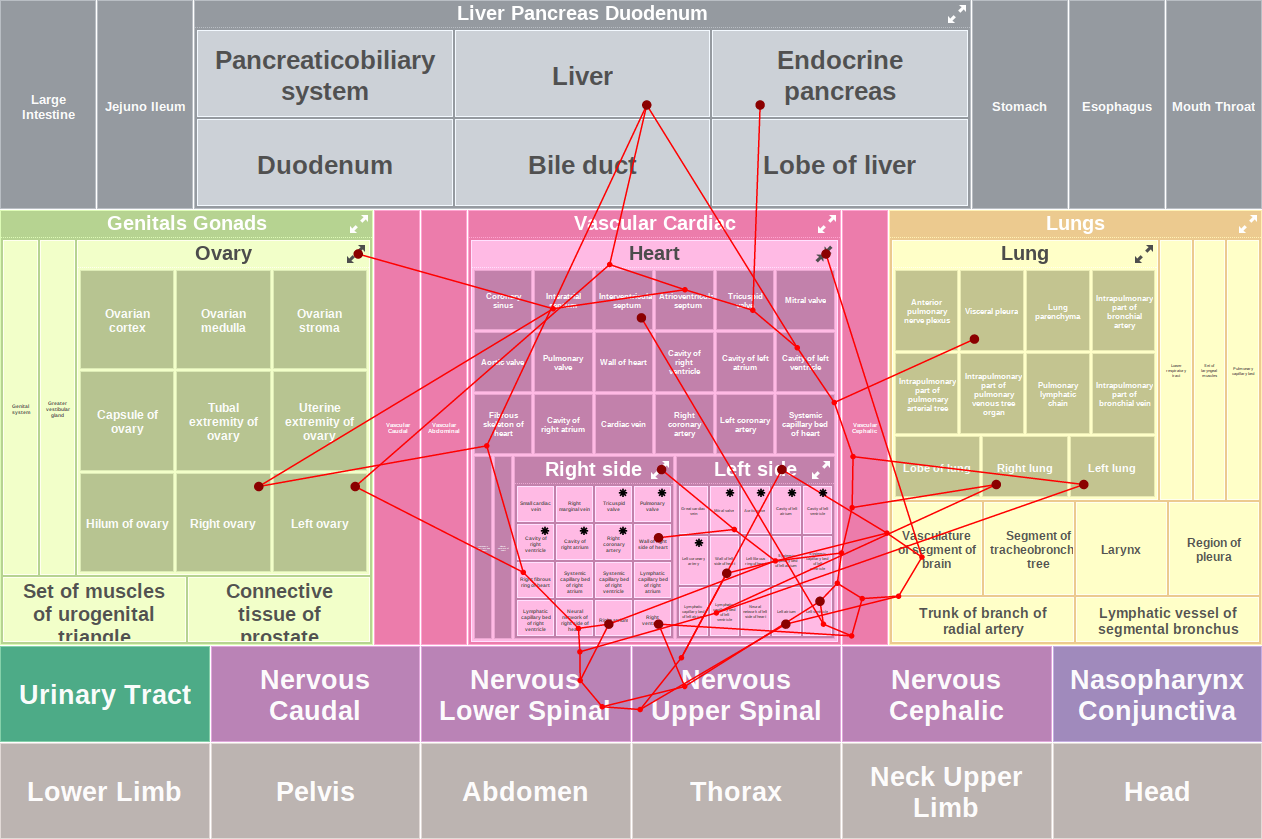
\includegraphics[width=5.8cm]{images/screenshot-bloodvessels.png}
    \label{fig:bloodvessels}
  }%
  \subfigure[Arterial connections from left ventricle]{
    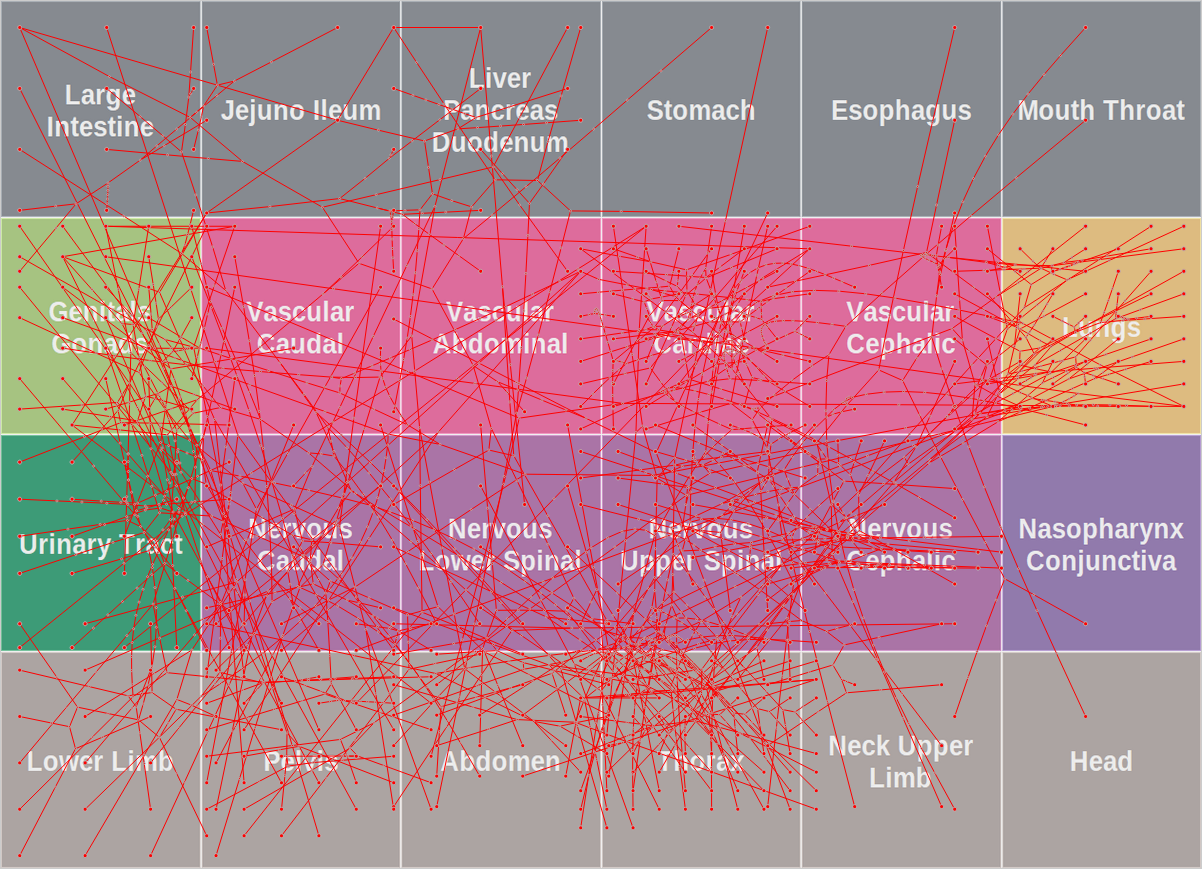
\includegraphics[width=5.8cm,height=3.855cm]{images/force-7101-new.png}
    \label{fig:force-7101}
  }\vskip-2mm
  \subfigure[Bundled connections from left ventricle]{
    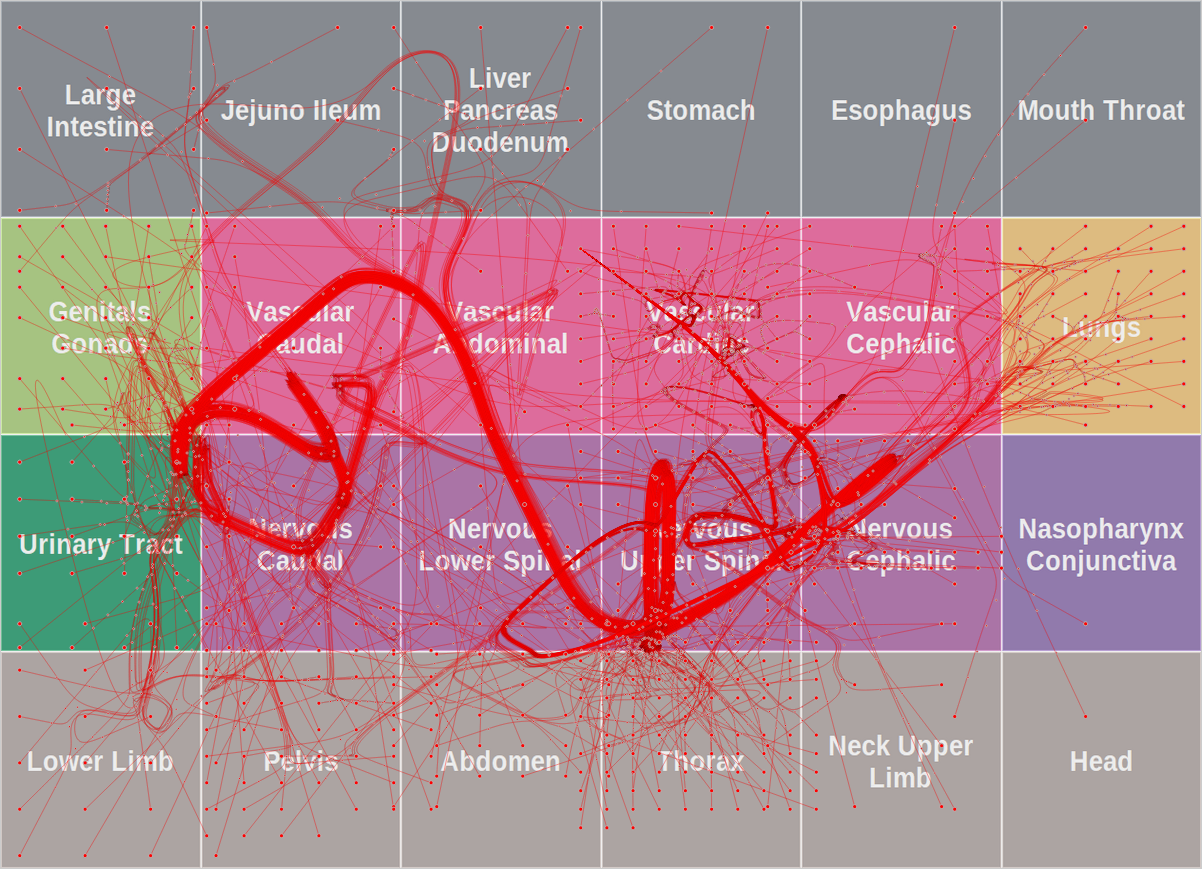
\includegraphics[width=5.8cm,height=3.855cm]{images/connections-7101-new.png}
    \label{fig:bundled-7101}
  }%
  \subfigure[Bundled connections to right atrium]{
    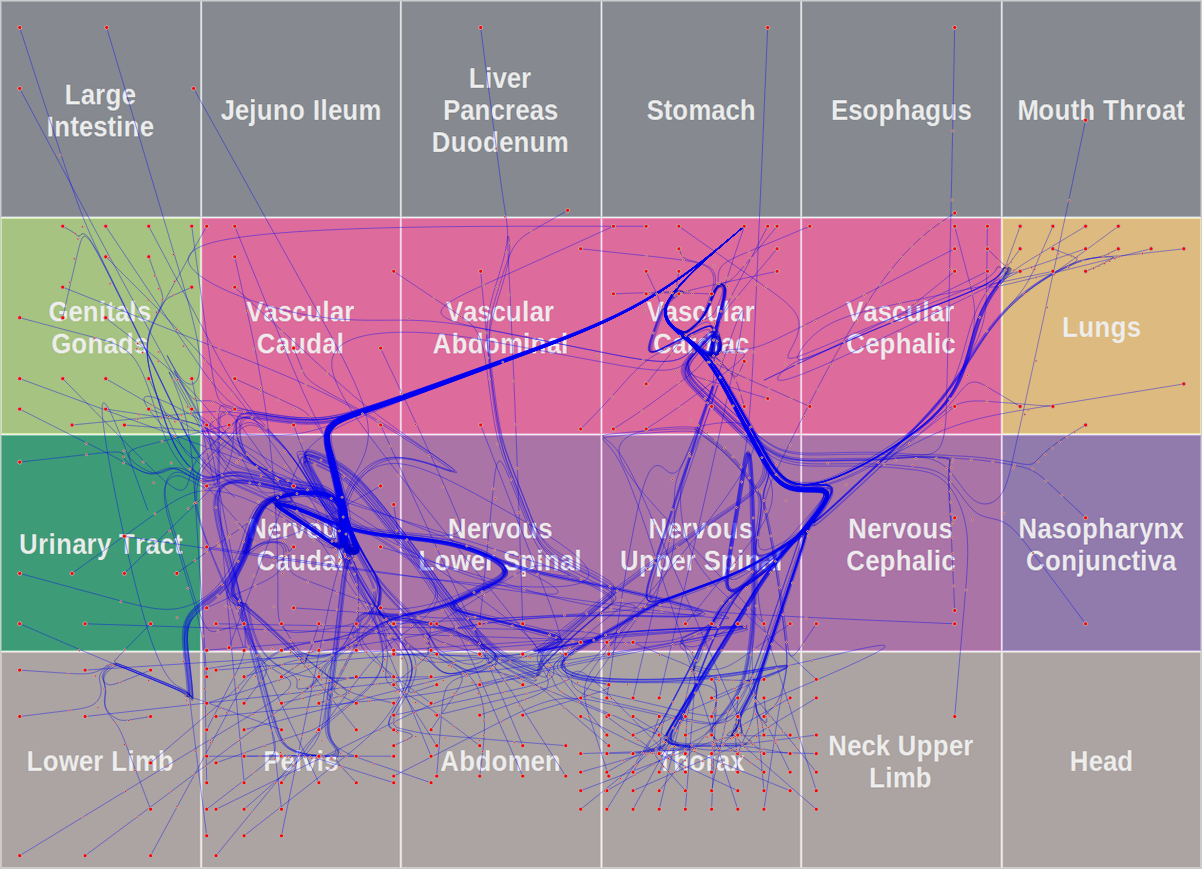
\includegraphics[width=5.8cm,height=3.855cm]{images/connections-7096b-new.png}
    \label{fig:bundled-7096}
  }\vskip1mm
  \caption{Overlaying cardiovascular connections. A straightforward
           approach works well when the number of connections is limited (a). When many
           connections need to be displayed, we quickly lose overview (b). This is
           mitigated by employing edge-bundling techniques (c,d).}
  \label{fig:vascular-connectivity}
\end{figure}

If there are too many edges to get a clear overview of the data ---as in \cref{fig:force-7101},
which shows the full connectivity graph for the left ventricle (7101) on the top-level body plan---
we can apply hierarchical edge bundling techniques that use path structure to bundle common sub-paths.
The result for the left ventricle is shown in \cref{fig:bundled-7101}, which gives a much nicer
overview. The result for the right atrium is shown in \cref{fig:bundled-7096}.

After a one-time pre-processing to import data from available external sources, we store connectivity data in a convenient format. A user can interact with and edit this data using the tool.


\subsection{Analyzing the Connectivity Data: an Example} %%%%%%%%%%%%%%%%%%%%%%%%%%%%%%%%%%%%%%%%%%%

Consider the blood vessels in the human body. Our initial dataset on this is a graph based on the FMA ontology, and consists of approximately 11,300 edges and over 10,000 distinct nodes. In this graph, an edge represents a flow process over an unbranched blood-vessel segment. Nodes represent blood vessel junctions and end-points. Samples of records from the dataset are shown in \cref{tab:vascular-connectivity}.

\begin{table}
	\def\vdt{\hskip1pt\vdots}
	\begin{tabular}{l@{\ }l@{\ }l@{\ }l@{\ }l@{\ }|@{\ }p{6.2cm}}
	  \textbf{Segment} & \textbf{T.} & \textbf{FMA} & \textbf{Node 1} & \textbf{Node 2} & \textbf{Description} \\
	  \hline
	  121a & 2    & 62528  & 62528\_2 & 62528\_4  & Arterioles in Microcirculation segment of Wall of left inferior lobar bronchus \\[.5mm]
	  121c & 2    & 62528  & 62528\_4 & 62528\_5  & Capillaries in Microcirculation segment of Wall of left inferior lobar bronchus\\[.5mm]
	  121v & 2    & 62528  & 62528\_3 & 62528\_5  & Venules in Microcirculation segment of Wall of left inferior lobar bronchus\\
	  \vdt & \vdt & \vdt   & \vdt     & \vdt      & \vdt  \\[.5mm]
	  8499 & 1    & 69333  & 8498\_0  & 62528\_2  & Arterial Segment 8499 of Trunk
	of left second bronchial artery from origin of supplying terminal segment
	to the arteriolar side of the Wall of left inferior lobar bronchus MC\\[.5mm]
	  9547 & 3 & 66699 & 9546\_0 & 62528\_3 & Venous Segment 9547 of Trunk of
	left bronchial vein from origin of supplying terminal segment to the
	venular side of the Wall of left inferior lobar bronchus MC
	\end{tabular}\vskip2mm
	\caption{Vascular connectivity data from the FMA ontology. The first column
	         is a unique segment identifier. The second shows the
	         type of a segment (1: arterial, 2: microcirculation, 3: venous,
	         and 4: cardiac chamber). The third contains FMA IDs. The fourth and
	         fifth contain identifiers of the two connected nodes.}
	\label{tab:vascular-connectivity}
\end{table}

A \emph{microcirculation (MC)} is represented by three edges connected in series: one representing tissue arterioles, a second for the bed of capillaries, and a third for the venules. In \cref{tab:vascular-connectivity}, the anatomical entity in which the MC is embedded is 62528 (``Wall of left inferior lobar bronchus''). The topology of its MC segment connectivity is as follows:
\[
	62528\_2  \;\xrightarrow{\;\text{121a}\;}\;
	62528\_4  \;\xrightarrow{\;\text{121c}\;}\;
	62528\_5  \;\xleftarrow {\;\text{121v}\;}\;
	62528\_3  \text.
\]
MC segment 121a is supplied with blood by the arterial segment 8499, and MC segment 121v is drained of blood by the venous segment 9547.

The accurate and comprehensible visualization of the cardiovascular system requires complex pre-processing; a biomedical expert in our team identified about 12 rules for the extraction of relevant data from the full dataset.
For illustration purpose, \cref{fig:vascular-connectivity} shows only paths connecting MCs of the walls of the heart (i.e., wall of left ventricle, left atrium, right ventricle or right atrium) to MCs belonging to the sub-organs of the tiles in our upper level 24 tile body plan. To obtain this view, we looked for the shortest paths --- due to the way the data is represented in the initial data set, cycles are possible. For example, the path from the left ventricle to the wall of left inferior lobar bronchus MC is
{$7101 \rightarrow 2406 \rightarrow \cdots \rightarrow 8499 \rightarrow 62528$,}
and the path from there to the right atrium is
{$7096 \leftarrow 771 \leftarrow \cdots \leftarrow 9546 \leftarrow 9547 \leftarrow 62528$.}

The first and the last IDs in this path correspond to the tiles in the treemap, while the intermediate IDs will be represented using auxiliary nodes with undefined coordinates. One of the issues we encountered is the need to determine optimal positions for these nodes. Since several paths can have common sub-paths, as shown in \cref{fig:bloodvessels}, the intermediate nodes should be positioned so as to minimize the overall path length. This motivates our application of the \emph{sticky force-directed graph visualization} method~\cite{FR91,Bos14} in which a sub-set of nodes have fixed coordinates, and the coordinates of the other nodes is determined by simulating imaginary forces applied by their edges.


\clearpage % Temporary, for better page/section alignment; TODO: REMOVE

%%%%%%%%%%%%%%%%%%%%%%%%%%%%%%%%%%%%%%%%%%%%%%%%%%%%%%%%%%%%%%%%%%%%%%%%%%%%%%%%%%%%%%%%%%
\section{Visualization of Models and Metadata} \label{sect:visualization2}               %
%%%%%%%%%%%%%%%%%%%%%%%%%%%%%%%%%%%%%%%%%%%%%%%%%%%%%%%%%%%%%%%%%%%%%%%%%%%%%%%%%%%%%%%%%%

The entities in the ApiNATOMY ontologies have various data associated with them, to which they are explicitly linked via semantic metadata annotations. This includes static and dynamic 3D models of body organs and their subsystems.
For instance, we extract and display neuronal reconstructions and associated metadata from \url{http://neuromorpho.org}~\cite{Asc06}.
\Cref{fig:neuron-big} shows a sample neuron model associated with the neocortex (reached through``Nervous Cephalic'' $\rightarrow$ ``Region of cerebral cortex'' $\rightarrow$ ``Neocortex''). ApiNATOMY allows users to show multiple 3D objects together in their proper context. For example, \cref{fig:neuron-small} shows a screenshot including the ``Neocortex'' neuron, as well as 3D models of the ``Liver'' and ``Stomach'', retrieved from BodyParts3D~\cite{MFT+09}.

\begin{figure}[t]
\centering
  \subfigure[A neuron in the ``Neocortex'']{
    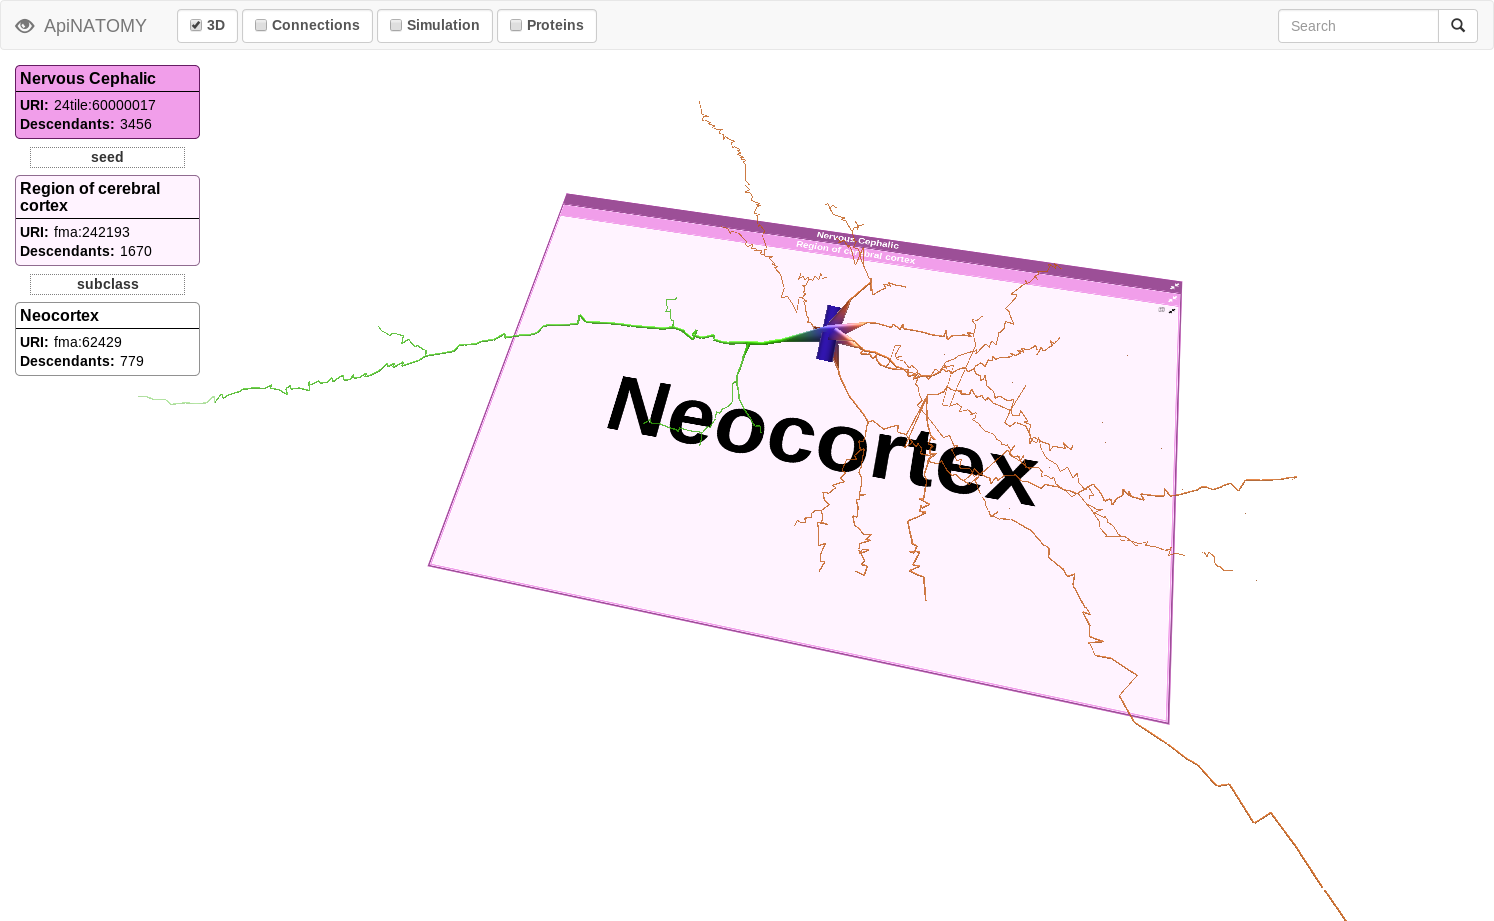
\includegraphics[width=5.4cm]{images/screenshot-neocortex-neuron.png}
    \label{fig:neuron-big}
  }
  \subfigure[Multiple 3D models in context]{
    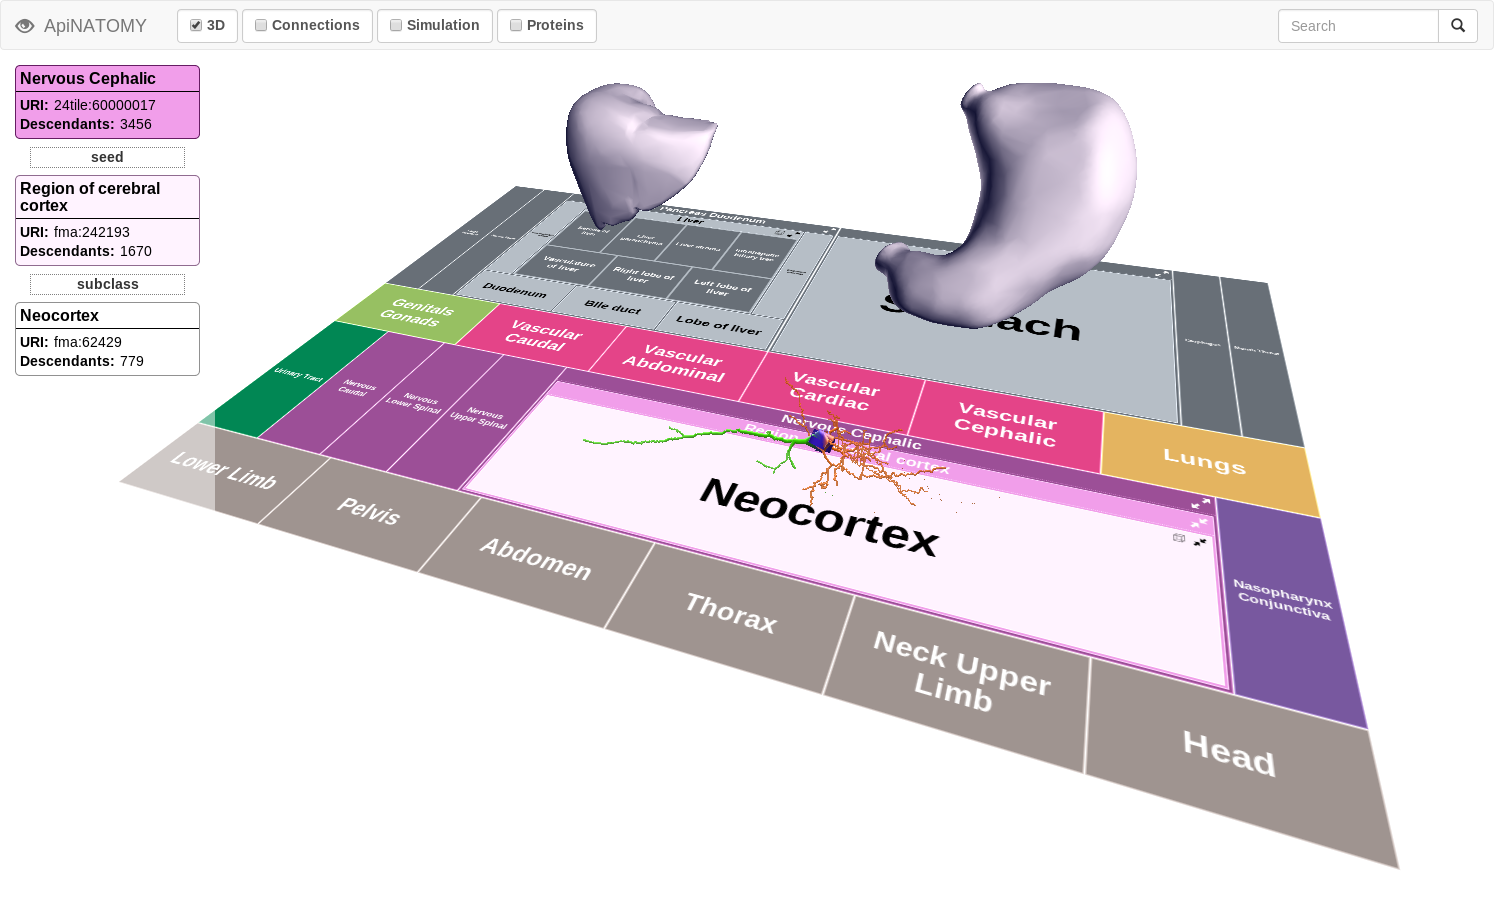
\includegraphics[width=5.4cm]{images/screenshot-3d-objects.png}
    \label{fig:neuron-small}
  }\vskip1mm
  \caption{Visualizing static 3D models}
  \label{fig:neurons}
\end{figure}

\begin{figure}[t]
\centering
%	\subfigure[Simulation control panel]{
%		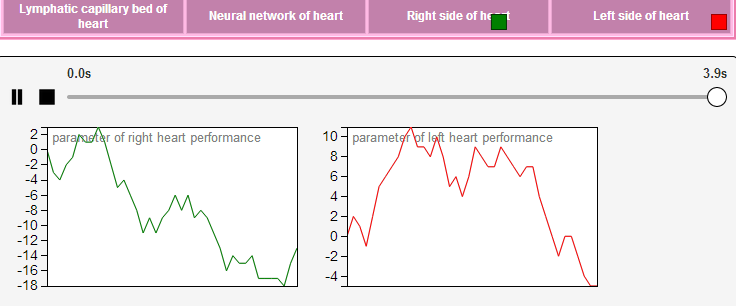
\includegraphics[width=5cm]{images/simulation.png}
%		\label{fig:panel}
%	}
	\subfigure[Protein interactions in 2D]{
		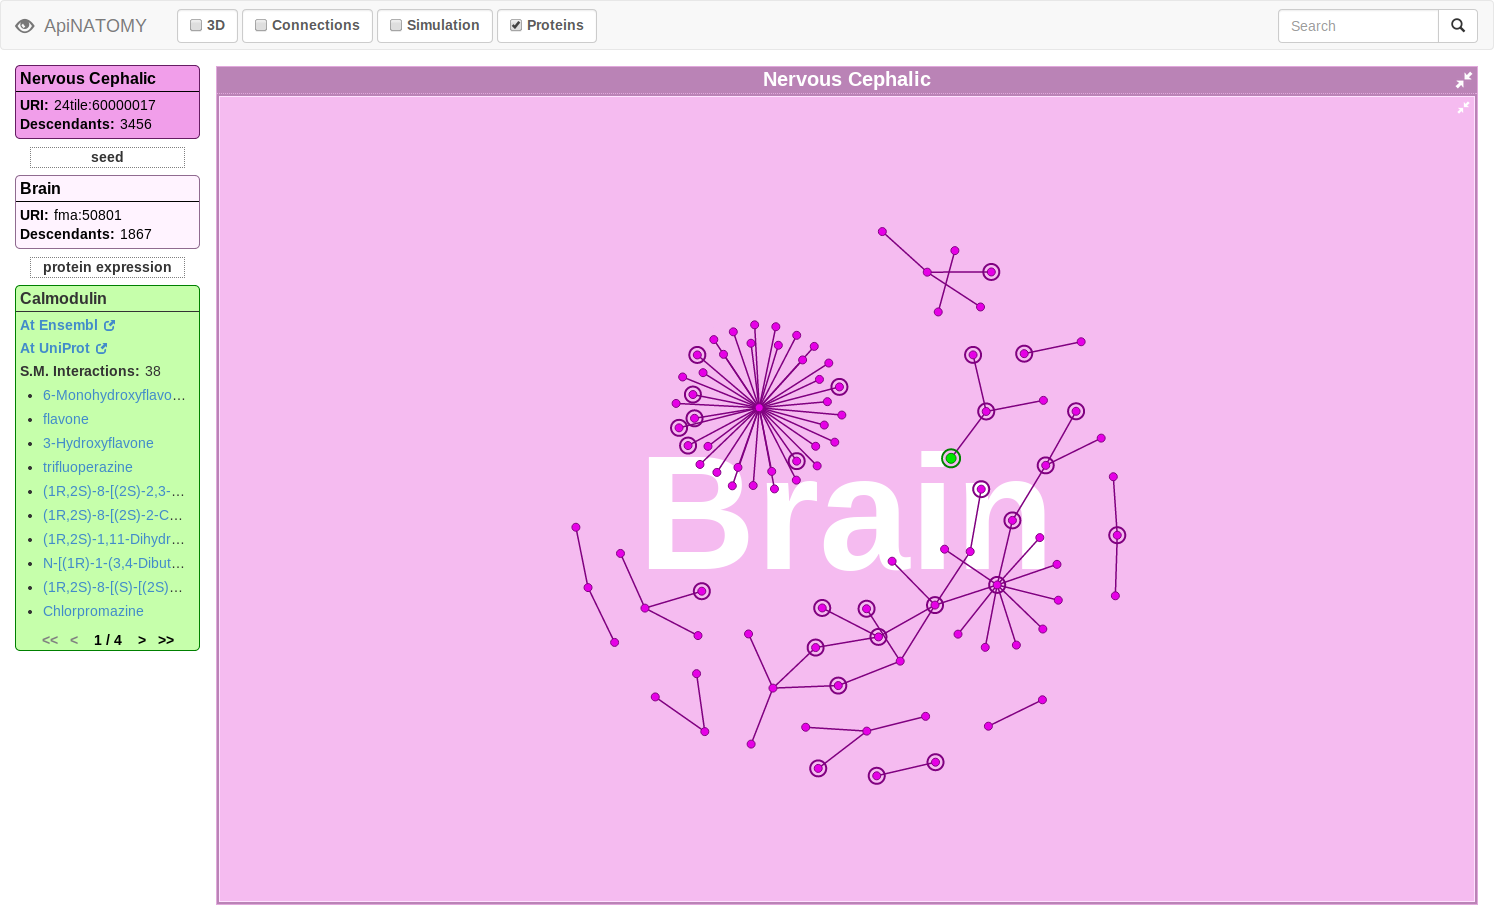
\includegraphics[width=5.4cm]{images/screenshot-proteins.png}
		\label{fig:protein}
	}
	\subfigure[Protein features in 3D]{
		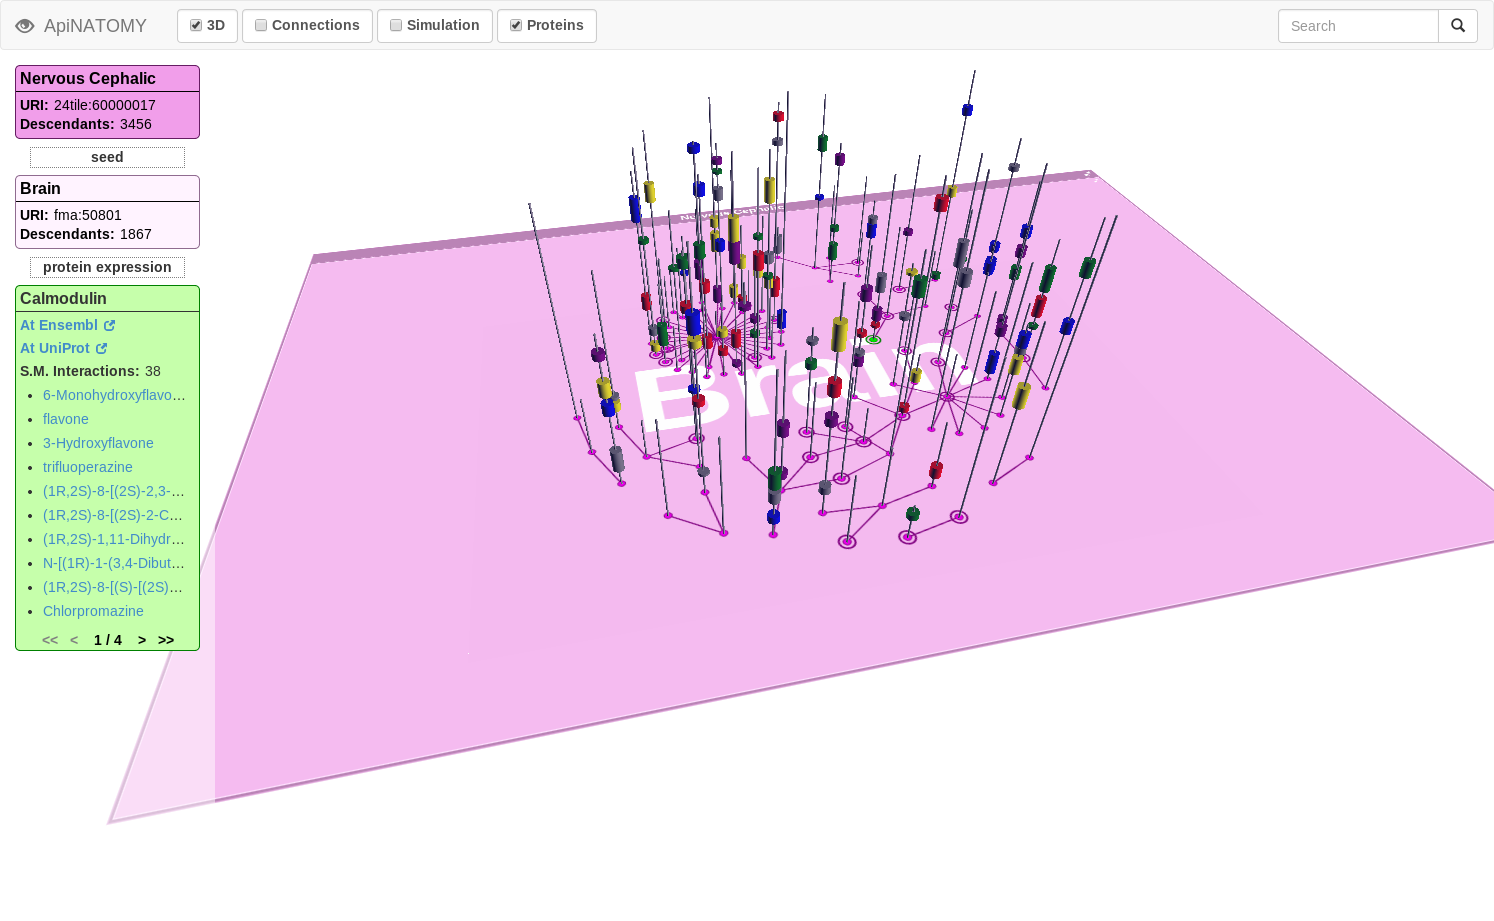
\includegraphics[width=5.4cm]{images/screenshot-proteins-3d.png}
		\label{fig:protein-3d}
	}\vskip1mm
	\caption{Visualizing protein expression, protein interaction and protein features}
	\label{fig:proteins}
\end{figure}

ApiNATOMY also supports the visualization of protein- and drug-interaction networks (\cref{fig:protein}) that are represented as graphs on top of treemap tiles. We are in the process of acquiring and integrating relevant data from the Ensembl genomic database~\cite{Ensemble}. In Ensembl, gene models are annotated automatically using biological sequence data (e.g. proteins, mRNA). We query this database to extract genes, transcripts, and translations with related protein features, such as PFAM domains. ApiNATOMY generates diagrams of protein-interactions and positions them on tiles where the corresponding genes are expressed. For easy access, protein diagrams are able to represent domain features in the form of color-coded 3D shapes extending from the circuitboard (\cref{fig:protein-3d}).

